%! Author = danielmendes
%! Date = 13.02.25

\chapter{Replikation}\label{ch:replikation}
In diesem Segment befassen wir uns mit dem Thema Replikation.
Replikation kann die Grundlage für den Aufbau großer, leistungsstarker Anwendungen auf der Basis von MySQL sein.
Es verfolgt dabei die sogenannte~\glqq Scale-Out\grqq-Architektur, bei der mehrere Storage-Knoten parallelisiert arbeiten (\cite{scale_out_eigenschaften}).
Nach außen hin wirkt es trotzdem wie ein einziges Gesamtsystem.
Bei dieser Architektur ist die Skalierbarkeit nahezu unbegrenzt, da man durch einfaches Hinzufügen weiterer Speicherknoten die Performance verbessern kann.
Im Gegensatz dazu ist Scale-Up durch die Systemgrenzen eines einzelnen Geräts limitiert.
Mit Scale-Out sind allerdings auch Nachteile verbunden, zu denen wir später in diesem Abschnitt kommen.
Wie schon in den vorherigen Kapiteln gehen wir zuerst auf die Grundlagen ein, dann betrachten wir die Konfiguration, die die Basis für die Benchmarks bilden und abschließend analysieren wir die Ergebnisse.

\section{Grundlagen}\label{sec:replication-grundlagen}
Replikation ermöglicht die Konfiguration eines oder mehrere Server als Replikate eines anderen Servers, auch Master genannt (\cite[pp. 447--477]{schwartz2012high}).
Sowohl die Begrifflichkeit Master-Replikat als auch die Varianten Primary-Secondary und Primary-Replica sind gebräuchlich.
Das grundlegende Problem, das die Replikation löst, besteht darin, die Daten eines Servers mit denen eines anderen synchron zu halten.
Es können sich mehrere Replikate mit einem einzigen Master verbinden und mit diesem synchron bleiben.
Außerdem können Master und Replikate in vielen verschiedenen Konfigurationen angeordnet werden.
Neben der klassischen Master-Replikat-Variante können Replikate selbst als Master für weitere Replikate dienen.
Zudem ist auch eine Master-Master-Kombination denkbar.
Die Vorteile der Replikation liegen nicht nur in einer höheren Effizienz, sondern auch in einer erhöhten Verfügbarkeit und besseren Skalierbarkeit.
Besonders gut ist es auch für Datenanalysen im Data Warehousing geeignet, aber Replikate sollte keine richtigen Backups ersetzten.
Die Effizienzvorteile gibt es insbesondere durch die Lastverteilung, bei der Leseanfragen auf mehrere Server verteilt werden.
Daher ist Replikation besonders für leselastige Anwendungen vorteilhaft ist.

Im folgenden Abschnitt erklären wir die Funktionsweise der Replikation und betrachten dabei den Fall mit einem Master und einem oder mehreren Replikaten.
Unmittelbar bevor jede Transaktion, die Daten aktualisiert, auf dem Master abgeschlossen wird, zeichnet der Master die Änderungen in seinem Binärlog (engl.\ binary log) auf.
MySQL schreibt die Transaktionen seriell ins Binary-Log und informiert die Storage Engines nach dem Schreiben der Ereignisse darüber, die Transaktionen zu committen.
Zu diesen Änderungen können beispielsweise neu deklarierte Tabellen oder Trigger sowie Einfügeoperationen in bestehende Tabellen gehören.
Im nächsten Schritt muss das Replikat die Veränderungen auf dem Master mitbekommen.
Dazu wird ein Worker-Thread gestartet, der als I/O-Replikations-Thread (engl.\ I/O-Slave-Thread) bezeichnet wird und eine Client-Verbindung zum Master öffnet (siehe Abbildung~\ref{fig:master-replica}).
Daraufhin wird ein spezieller Prozess gestartet, der die Ereignisse aus dem Binary-Log des Masters liest (engl.\ binlog dump process).
Nach dem Verarbeiten schreibt der Thread die Werte auf seine eigene Festplatte in das sogenannte Relay-Log.
Wenn er alle Ereignisse auf dem Log verarbeitet hat, geht er in einen passiven Zustand und wartet auf Aktualisierungen.
Den letzten Teil des Prozesses übernimmt der SQL-Slave-Thread.
Dieser liest und spielt Ereignisse aus dem Relay-Log ab und aktualisiert so die Daten der Replikate, sodass sie mit denen des Masters übereinstimmen.
Wenn beide Threads eine etwa gleich schnelle Verarbeitung haben, dann bleibt das Relay-Log normalerweise im Cache des Betriebssystems und es gibt nur sehr geringe Mehrkosten (engl.\ Overhead).
Die Ereignisse, die der SQL-Thread ausführt, können optional zusätzlich in das eigene Binary-Log der Replikate geschrieben werden.

\vspace{-5pt}
\begin{figure}[H]
  \centering
  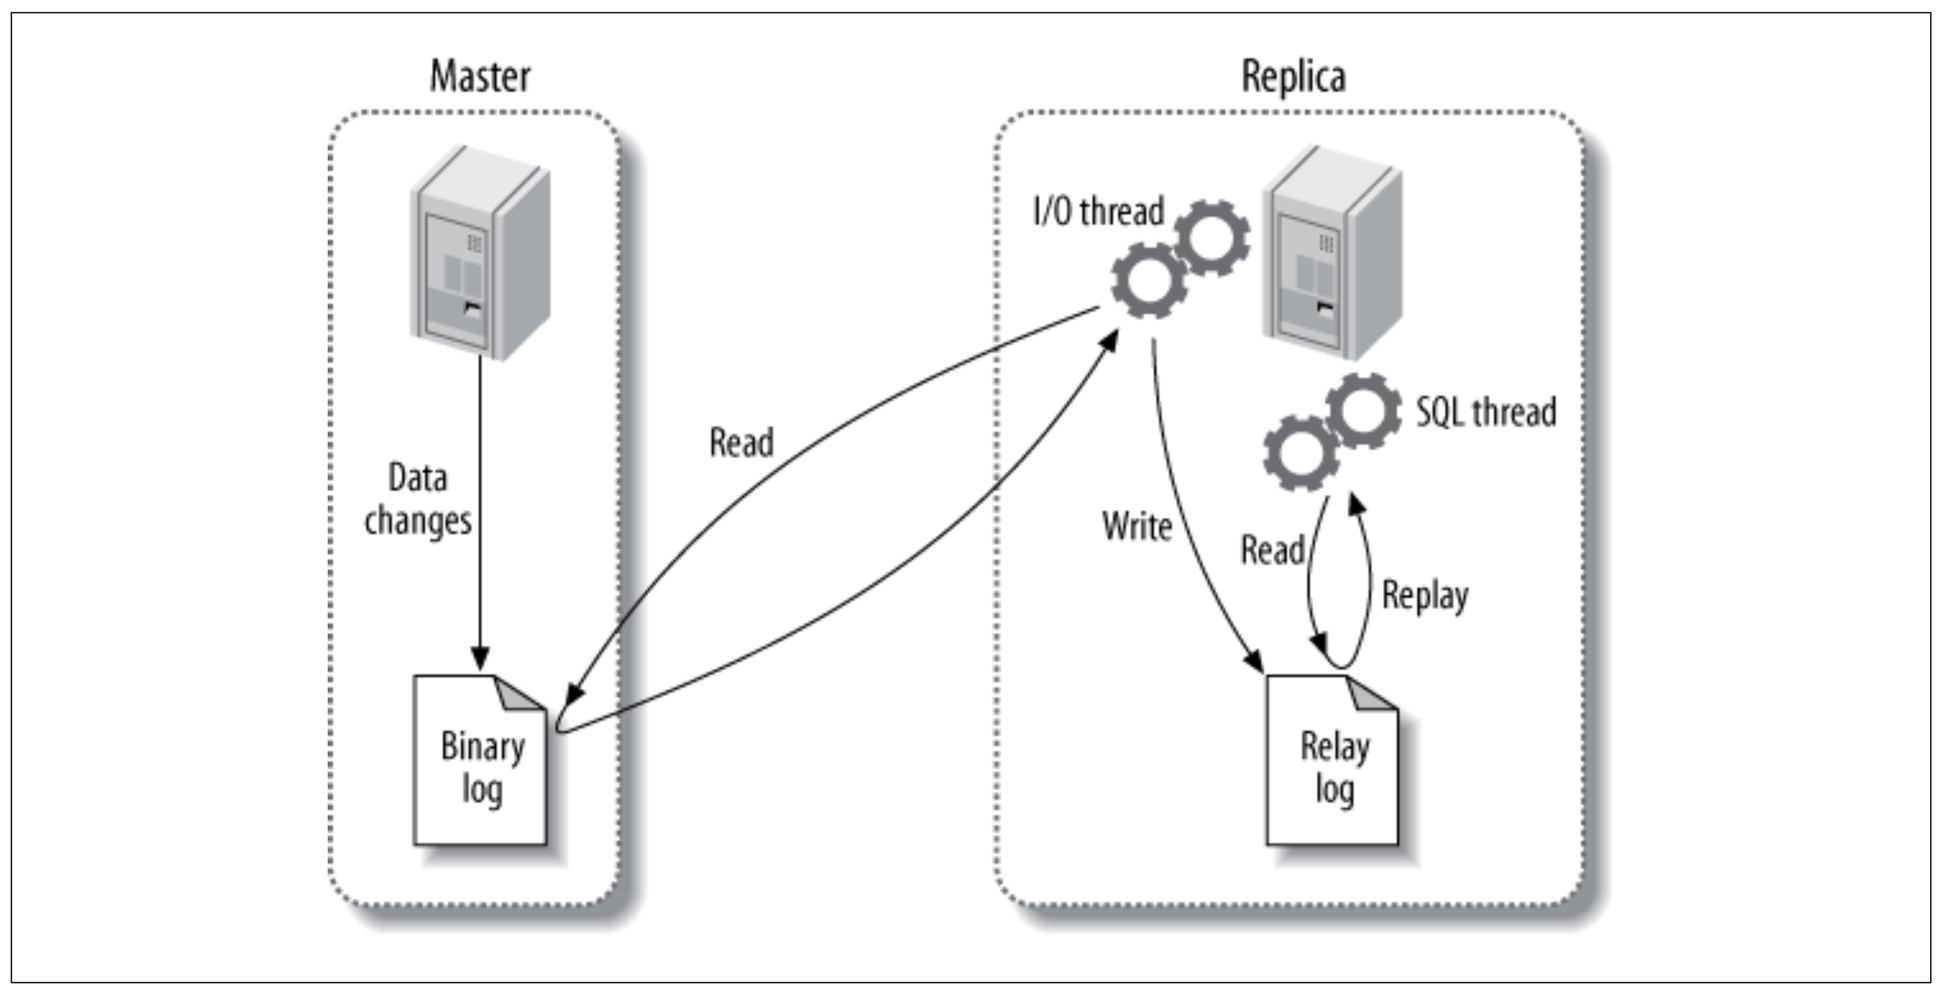
\includegraphics[width=.8\textwidth]{PNGs/Textbook/Master_Replica}
  \caption[Master-Replikat-Visualisierung]{Darstellung der unterschiedlichen Threads}
  \label{fig:master-replica}
\end{figure}
\vspace{-18pt}

Die Abbildung~\ref{fig:master-replica} zeigt nur die beiden Replikation-Threads, die auf dem Replikat laufen.
Zusätzlich gibt es jedoch einen weiteren Thread auf dem Master, der die vom Replikat zum Master geöffnete Verbindung auf dem Master startet.

Die Replikationsarchitektur entkoppelt die Prozesse des Abrufens und Schreiben von Ereignissen auf dem Replikat.
Dadurch können die beiden Threads asynchron arbeiten, sodass der I/O-Thread unabhängig vom SQL-Thread agieren kann.
Dies hat jedoch zur Folge, dass Änderungen, die auf dem Master parallel in verschiedenen Threads ausgeführt werden könnten, auf dem Replikat nicht parallelisiert werden können.
Das liegt daran, dass die Veränderungen auf dem Replikat in einem einzigen Thread abgearbeitet werden.
Generell gibt es keine Garantie für die Latenz auf des Replikats und große Abfragen können dazu führen, dass das Replikat Sekunden, Minuten oder sogar Stunden hinter dem Master zurückbleibt.
Der Flaschenhals (engl.\ bottleneck) des gesamten Systems stellt die Anzahl der Schreibvorgänge dar, die der langsamste Thread ausführen kann.

Die Replikation verursacht nur einen geringen Mehraufwand für den Master.
Wenn das binäre Logging für Backups und Point-in-Time-Recovery genutzt wird, kann es jedoch deutlich mehr Ressourcen beanspruchen.
Jedes angeschlossene Replikat verursacht nur eine geringe zusätzliche Last (hauptsächlich Netzwerk-I/O) auf dem Master.
Trotzdem sollten die Auswirkungen vieler Replikate nicht unterschätzt werden, da sie im Wesentlichen zu unnötiger Daten-Duplikation führen.

Als Nächstes betrachten wir die zwei verschiedenen Arten der Replikation, die von MySQL unterstützt werden: die anweisungsbasierte (engl.\ statement-based) und die zeilenbasierte (engl.\ row-based) Replikation.
Die anweisungsbasierte Replikation wird seit MySQL 5.0 und älter unterstützt und funktioniert, indem die Abfrage, die die Daten auf dem Master geändert hat, protokolliert wird.
Wenn ein Replikat das Ereignis aus dem Relay-Log liest und ausführt, wird die tatsächliche SQL-Abfrage erneut ausgeführt, die der Master ausgeführt hat.
Der offensichtlichste Vorteil davon ist, dass sie relativ einfach zu implementieren ist und das Protokollieren sowie Wiederholen der Anweisungen das Replikat logischerweise mit dem Master synchron halten sollte.
Außerdem sind die Binary-Log-Ereignisse in der Regel recht kompakt sind und verbrauchen nicht viel Bandbreite.
In der Praxis gibt es jedoch Änderungen auf dem Master, die von Faktoren abhängen, die über den reinen Abfragetext hinausgehen.
Beispielsweise werden Anweisungen zu leicht oder sogar deutlich unterschiedlichen Zeiten auf dem Master und dem Replikat ausgeführt.
Deshalb muss das Binary Log nicht nur den Abfragetext, sondern auch Metadaten wie den aktuellen Zeitstempel enthalten.
Einige Anweisungen kann MySQL nicht korrekt replizieren, wie zum Beispiel Abfragen, die die Funktion CURRENT\_USER() verwenden.
Auch gespeicherte Routinen und Trigger stellen bei dieser Art der Replikation ein Problem dar.

Die zeilenbasierte Replikation speichert die tatsächlichen Datenänderungen im Binary-Log.
Ein großer Vorteil, der daraus folgt, ist, dass MySQL jede Anweisung korrekt replizieren kann.
Zudem können einige Änderungen mithilfe der zeilenbasierte Replikation effizienter sein, da das Replikat die Abfragen, die die Zeilen auf dem Master geändert haben, nicht erneut ausführen muss.
Zum Beispiel, wenn eine Abfrage viele Zeilen in der Quelltabelle scannt, aber nur drei Zeilen in der Zieltabelle bearbeitet.
Bei der anweisungsbasierten Replikation müsste ein Replikat die Anweisung erneut ausführen, nur um ein paar Zeilen zu erstellen, während dies bei der zeilenbasierten Replikation effizient und trivial ist.
Andererseits ist das folgende Ereignis deutlich günstiger mit statement-basierter Replikation zu replizieren:

\vspace{-5pt}
\begin{lstlisting}[language=SQL]
UPDATE master_table SET col1 = 0;
\end{lstlisting}
\vspace{-5pt}

Die Verwendung der zeilenbasierten Replikation für diese Abfrage wäre sehr teuer, da jede Zeile geändert und somit ins Binary-Log geschrieben wird.
Dadurch würde das Binary-Log-Ereignis extrem groß werden, was sowohl beim Protokollieren als auch bei der Replikation zu einer höheren Last auf dem Master führen würde.
Damit kommen wir zu weiteren Vor- und Nachteilen der unterschiedlichen Arten.

Die anweisungsbasierte Replikation eignet sich besser, wenn das Schema auf Master und Replikat unterschiedlich ist und unterstützt Szenarien mit unterschiedlichen, aber kompatiblen Datentypen oder Spaltenreihenfolgen.
Zudem erleichtert sie Schemaänderungen auf Replikaten, die später als Master dienen sollen, wodurch Ausfallzeiten reduziert werden können.
Im Gegensatz dazu kann die zeilenbasierte Replikation bei Schemaänderungen auf einem Replikat bestimmte Operationen nicht ausführen, bietet jedoch eine zuverlässige Funktionalität mit allen SQL-Konstrukten.
Sie stopp auch bei Fehlern, z.B.\ wenn eine erwartete Zeile auf dem Replikat fehlt und weist damit auf Inkonsistenzen hin, während der andere Typ keine Hinweise auf fehlende Einträge gibt.
Die Fehlersuche und das Verständnis von Problemen sind bei der anweisungsbasierten Replikation einfacher, da die Änderungen über verständliche SQL-Anweisungen erfolgen.
Bei der zeilenbasierten Replikation ist die Nachvollziehbarkeit der Änderungen dagegen schwieriger, jedoch gibt es dafür weniger Locking-Probleme.
Die zeilenbasierte Replikation erleichtert die Datenwiederherstellung durch das Speichern alter Daten, wobei eine Wiederherstellung zu einem bestimmten Zeitpunkt mit einem Binary-Log im zeilenbasierten Format zwar schwieriger, aber möglich ist.
Außerdem benötigt sie häufig weniger CPU-Ressourcen, da keine komplexe SQL-Ausführungslogik erforderlich ist.

Da kein Format in jeder Situation perfekt ist, kann MySQL dynamisch zwischen statement-basierter und row-basierter Replikation wechseln.
Standardmäßig wird die statement-basierte Replikation verwendet, aber wenn MySQL ein Ereignis erkennt, das nicht korrekt als Statement repliziert werden kann, wechselt es automatisch zur row-basierten Replikation.
Alternativ kann das Format auch durch Setzen der Variable \texttt{binlog\_format} manuell gesteuert werden.

\section{Konfiguration des Master-Replikat-Ansatzes}\label{sec:replication-konfiguration}

Damit wir Benchmarks ausführen können, müssen den Master-Replika-Ansatz in MySQL konfigurieren.
Zunächst müssen wir festlegen, welches Szenario der Replikation wir umsetzen wollen.
In diesem Kapitel betrachten wir das Modell mit einem Master und einer beliebigen Anzahl an Replikaten.
Die erforderlichen Schritte umfassen das Erstellen der Master- und Replikationsknoten und der anschließenden Anweisung an das Replikat, sich mit dem Master zu verbinden.
Abschließend muss die Replikation gestartet werden.
Nach dem Erstellen der Knoten müssen wir uns mit einigen speziellen MySQL-Privilegien befassen, die erforderlich sind, damit die Replikationsprozesse ordnungsgemäß ausgeführt werden können.
Dazu muss ein Benutzer auf dem Master erstellt werden und diesem die richtigen Privilegien zugewiesen werden, damit der I/O-Thread sich als dieser Benutzer verbinden und das Binary-Log des Masters lesen kann.
Außerdem dürfen wir nicht vergessen, die Datenbank zu erstellen, auf der die Benchmarks ausgeführt werden (wie in~\ref{lst:tools-create-db}).

\vspace{-7pt}
\begin{lstlisting}[language=SQL,caption=Datenbank- und Nutzererstellung sowie Rechtevergabe,label={lst:replication-privileges}]
CREATE DATABASE sbtest;
CREATE USER 'repl'@'%' IDENTIFIED WITH sha256_password BY 'repl_password';
GRANT REPLICATION SLAVE ON *.* TO 'repl'@'%';
\end{lstlisting}
\vspace{-5pt}

Den Nutzer müssen wir nur auf dem Master erstellen, aber wir benötigen ihn auch bei der Verbindung der Replikate mit dem Master.
Im nächsten Schritt müssen einige Einstellungen auf dem Master und den Replikaten vorgenommen werden.
Zum einen muss die Binärprotokollierung aktiviert und zum anderen eine einzigartige ID mit dem Parameter \texttt{server\_id} angegeben werden.
Wenn die Binärprotokollierung in der Konfigurations-Datei nicht bereits angegeben wurde, muss MySQL neu gestartet werden.
Alternativ können die Einstellungen auch direkt beim Starten des Containers angegeben werden.
Um zu überprüfen, ob die Binary-Logdatei auf dem Master erstellt wurde, kann man abhängig von der MySQL-Version folgende Befehle ausführen:

\vspace{-7pt}
\begin{lstlisting}[language=SQL,caption=Anzeige der Konfiguration,label={lst:replication-master-config},style=custom_daniel]
SHOW BINARY LOG STATUS; --MySQL ≥8.0.23
SHOW MASTER STATUS; --MySQL <8.0.23
\end{lstlisting}
\vspace{-5pt}

Die wichtigste Einstellung für das Binär-Logging auf dem Master ist \texttt{sync\_binlog}, wobei der Wert \texttt{1} gesetzt werden muss.
Diese Option sorgt dafür, dass MySQL den Inhalt des Binary-Logs, bei jedem Transaktions-Commit auf die Festplatte synchronisiert.
Ist die Option deaktiviert, verringert sich der Arbeitsaufwand des Servers, jedoch könnten Binary-Log-Einträge bei einem Absturz verloren gehen.
Auf einem Replikat, das nicht als Master dient, erzeugt diese Option unnötigen Mehraufwand.
Außerdem wird empfohlen, einen Basisnamen für das Binary-Log explizit anzugeben, um einheitliche Namen auf allen Servern zu gewährleisten und Änderungen bei einem Hostnamenwechsel zu vermeiden.
Dazu muss ein Argument für die \texttt{log\_bin}-Option angegeben werden.

Es gibt noch weitere optionale Konfigurationsparameter, die wir hinzufügen können.
Einer davon ist der Parameter \texttt{relay\_log}, der den Speicherort und den Namen des Relay-Logs festlegt.
Ein weiterer wichtiger Parameter ist \texttt{log\_slave\_updates}, der es dem Replikat ermöglicht, replizierte Ereignisse in sein eigenes Binary-Log zu schreiben.
Die Option \texttt{skip\_slave\_start} sorgt dafür, dass das Replikat nach einem Absturz automatisch startet, was die Möglichkeit offenlässt, den Server im Falle eines Problems zu reparieren.
Zudem sorgt die Option \texttt{read\_only} dafür, dass die meisten Benutzer keine nicht-temporären Tabellen ändern können.
Die einzigen Ausnahmen bilden der Replikation-SQL-Thread und Threads mit dem \texttt{SUPER}-Privileg, weshalb dieses Privileg normalen Benutzern nicht zugewiesen werden sollte.
In unserem Anwendungsfall haben die Replikate die Option \texttt{read\_only} aktiviert.
Wenn das Replikat stark im Rückstand ist, kann der I/O-Thread den Festplattenspeicher füllen.
Mit der Option \texttt{relay\_log\_purge} kann verhindert werden, dass der Replikation-SQL-Thread diese entfernt diese, sobald er mit deren Verarbeitung fertig ist.

Der nächste Schritt besteht darin, dem Replikat mitzuteilen, wie es sich mit dem Master verbinden und dessen Binary-Logs abspielen kann.
Umgesetzt kann das mit der Ausführung des folgenden Befehls auf allen Replikaten:

\vspace{-8pt}
\begin{lstlisting}[language=SQL,caption=Verbindung des Replikats zum Master,label={lst:replication-connection-replica-master}]
CHANGE MASTER TO
  MASTER_HOST='YOUR_HOST_NAME',
  MASTER_USER='YOUR_USER',
  MASTER_PASSWORD='YOUR_PASSWORD',
  MASTER_LOG_FILE='mysql-bin.000001',
  MASTER_LOG_POS=0;
\end{lstlisting}
\vspace{-5pt}

Die Spalten \texttt{MASTER\_LOG\_FILE} und \texttt{MASTER\_LOG\_POS} müssen mit dem Ergebnis von dem Befehl aus~\ref{lst:replication-master-config} übereinstimmen.
Um sicherzustellen, dass die Datenbank \texttt{sbtest} und der Benutzer mit den entsprechenden Privilegien tatsächlich existieren, müssen wir den Befehl aus~\ref{lst:replication-master-config} bereits vor der Ausführung des Befehls in~\ref{lst:replication-privileges} durchführen.
Um die eigentliche Replikation zu starten, muss man den folgenden Befehl auf den Replikaten ausführen:

\vspace{-8pt}
\begin{lstlisting}[language=SQL,caption=Starten der Replikation,label={lst:replication-replica-start}]
START SLAVE;
\end{lstlisting}
\vspace{-5pt}

Mit dem folgenden Befehl lässt sich überprüfen, ob die Durchführung erfolgreich war:

\vspace{-8pt}
\begin{lstlisting}[language=SQL,caption=Status des Replikats,label={lst:replication-replica-status}]
SHOW PROCESSLIST\G;
\end{lstlisting}
\vspace{-5pt}

Die Spalten \texttt{Slave\_IO\_State}, \texttt{Slave\_IO\_Running} und \texttt{Slave\_SQL\_Running} zeigen an, ob die Replikationsprozesse laufen oder nicht.
Wenn \texttt{Seconds\_Behind\_Master} nicht mehr NULL ist, bedeutet das, dass der I/O-Thread bereits alle Binary-Logs abgerufen hat und nun auf ein Ereignis vom Master wartet.
Man sollte auch beobachten können, dass die verschiedenen Datei- und Positionswerte auf dem Replikat inkrementiert werden, wenn man Änderungen an dem Master vornimmt.
Außerdem sollten zwei Threads auf dem Replikat aktiv sein, die unter dem Benutzer~\glqq system user\grqq laufen.

Bei den bisherigen Setup-Anweisungen sind wir von einer frischen Installation ausgegangen.
Es gibt aber auch andere Möglichkeiten, um ein Replikat von einem anderen Server zu initialisieren.
Zum einen kann man bereits existierende Daten von einem Master kopieren, ein Replikat von einem anderen Replikat klonen oder ein Replikat aus einem aktuellen Backup starten.
Um ein Replikat mit einem Master zu synchronisieren, sind drei Elemente erforderlich: eine Momentaufnahme der Master-Daten zu einem bestimmten Zeitpunkt, die Log-Datei des Masters mit dem entsprechenden Byte-Offset (ermittelbar durch den Befehl~\ref{lst:replication-master-config}) sowie die Binary-Logs des Masters ab diesem Zeitpunkt.
Eine kalte Kopie erfordert das Herunterfahren des Masters, um dessen Dateien zu kopieren, bevor er mit einem neuen Binary-Log neu gestartet wird, was jedoch zu Ausfallzeiten führt.
Bei einer warmen Kopie können die Dateien übertragen werden, während der Server weiterhin läuft.

\section{Analyse}\label{sec:replication-analyse}

Im vorherigen Abschnitt wurde erklärt, wie man den Master und vor allem die Replikate korrekt konfiguriert und den Prozess der Replikation startet.
Für die Durchführung der Benchmarks benötigen wir wieder die Kundentabelle und die Bestelltabelle aus Kapitel~\ref{sec:projektaufbau-mit-beispiel}.
Die einzigen erforderlichen Anpassungen betreffen das Festlegen des Binlog-Formats, das über die Variable \texttt{binlog\_format} definiert wird und die Werte \texttt{STATEMENT}, \texttt{ROW} oder \texttt{MIXED} annehmen kann.
Diese Einstellung kann entweder global für den gesamten Server oder lokal für die aktuelle Sitzung mithilfe des Befehls \texttt{SET SESSION} geändert werden.
Damit können wir die Performanceunterschiede zwischen den einzelnen Arten, insbesondere für die Einfügeoperationen, vergleichen.
Der eigentliche Aufwand bei diesen Benchmarks besteht in der Einrichtung der Replikation auf dem lokalen Rechner und im Workflow, während die Veränderungen an den Lua-Skripten minimal sind.

Im ersten Vergleich wollen wir die Performanceunterschiede zwischen dem Master-Replikat-Ansatz und dem Ansatz mit einem MySQL-Server feststellen.
Beim Master-Replikat-Ansatz verwenden wir mit \texttt{ROW} immer den Default-Wert des Binlog-Formats.
Damit keine Fehler auftreten, müssen wir die beiden Ansätze miteinander kompatibel machen.
Das Problem dabei ist, dass der Standardport von MySQL (3306) nicht gleichzeitig verwendet werden darf.
Daher starten wir den Master auf Port 3307 und jedes Replikat erhöht diesen Wert um 1.
Somit nutzt das dritte Replikat den Port 3310.
Die Anzahl an Replikate können wir in der \texttt{envs.json}-Datei mithilfe der Variablen \texttt{REPLICAS\_COUNT} festlegen.
Die Voraussetzung dafür ist, dass es lokal mindestens diese Anzahl an gestarteten und konfigurierten Replikate gibt.
Innerhalb des Workflowjobs muss nichts anpasst werden, da dort \texttt{REPLICAS\_COUNT} dazu genutzt wird, die exakte Anzahl an Replikate zu starten.
Wichtig ist noch zu erwähnen, dass die Insert-Befehle nur auf dem Master, also Port 3307, ausgeführt werden.
Die Select-Befehle werden sowohl auf dem Master als auch auf die Replikate ausgeführt.

Wenn wir die Ergebnisse aus Abbildung~\ref{fig:replication-vs-no} betrachten, dann fällt auf, dass die Version ohne Replikation am schnellsten ist.
Danach folgen die Readabfragen auf dem Master auf Port 3307.
Der Unterschied der beiden liegt bei etwa 15\%.
Nah an dem Ergebnis vom Master ist das erste Replikat (3308).
Überraschenderweise folgen mit etwas mehr Abstand erst die anderen beiden Replikate auf den Ports 3309 und 3310.
Die Schreibgeschwindigkeit ist sehen wir einen deutlichen Unterschied zwischen den beiden Varianten, da durch den Prozess der Replikation die Schreibgeschwindigkeit ungefähr 60\% langsamer ist.

\vspace{-8pt}
\begin{figure}[H]
  \centering
  \begin{subfigure}[t]{0.48\textwidth}
    \centering
    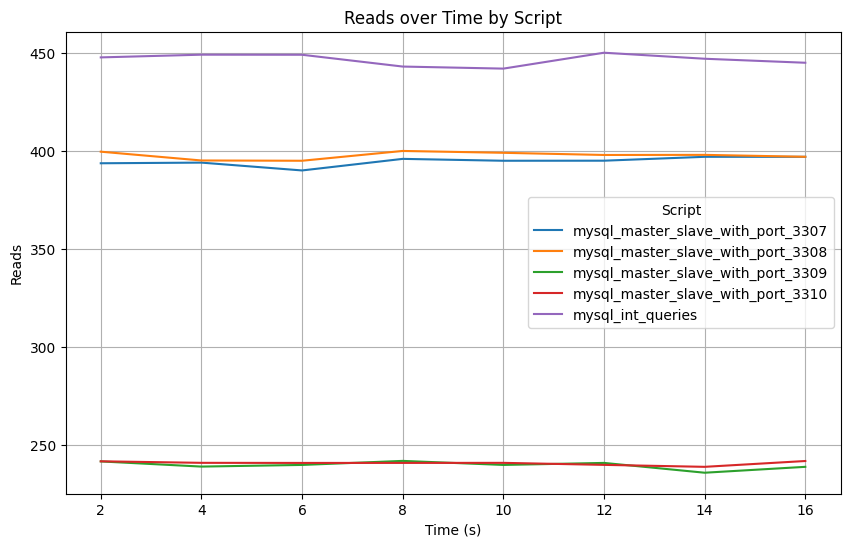
\includegraphics[width=\textwidth]{PNGs/Script/Replication/replication-vs-no/Reads}
  \end{subfigure}
  \hfill
  \begin{subfigure}[t]{0.48\textwidth}
    \centering
    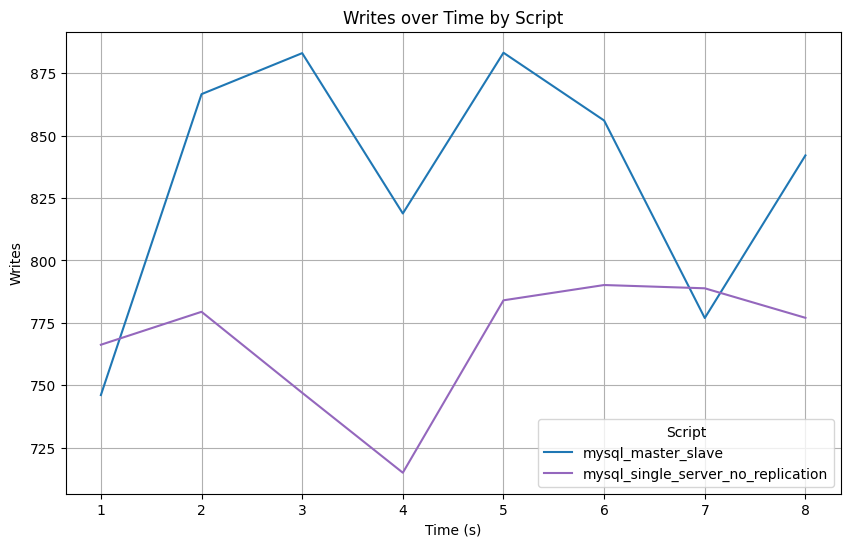
\includegraphics[width=\textwidth]{PNGs/Script/Replication/replication-vs-no/Writes}
  \end{subfigure}
  \vspace{-8pt}
  \caption[Replikation: Master-Replikat-Ansatz vs Single-Server]{Vergleich zwischen Master mit 3 Replikaten und Single-Server-Ansatz }
  \label{fig:replication-vs-no}
\end{figure}
\vspace{-20pt}

Bei dem ersten Vergleich betrug der Threads-Wert bei Einfügungen und Abfragen \texttt{1}, sodass die Leistung eines einzelnen Threads ersichtlich wurde.
Aus den Ergebnissen können wir schlussfolgern, dass der Single-Server am effizientesten ist, solange er nicht stark ausgelastet ist.
In dem Fall bringt der Master-Replikat-Ansatz demnach keine Vorteile.
Anders sieht das aus, wenn wir die Last auf den Server erhöhen, indem wir die Anzahl der Threads erhöhen.
Die Threadanzahl kann beim Aufführen des Sysbench-Befehls mit dem Parameter \texttt{--threads} festgelegt werden.
Die Prozesse sollen die Last durch Nutzer in der Datenbank simulieren.
Um den Vergleich zwischen dem Single-Server und dem Master-Replikat-Ansatz zu verdeutlichen, führen wir den Benchmark mit 8 und 16 Threads durch.
Beim Single-Server werden alle Threads auf einem Server ausgeführt, während sie beim Master-Replikat-Ansatz auf den Master und die drei Replikate gleichmäßig aufgeteilt werden.
Bei 8 Threads wird die Last so aufgeteilt, dass der Master und jedes Replikat 2 Threads verarbeitet ($4 * 2 = 8$).
Nach diesem Prinzip lassen wir den Benchmark auch mit 16 Threads durchführen (siehe Abbildung~\ref{replication-multiple-select-threads-reads}).

\vspace{-8pt}
\begin{figure}[H]
  \centering
  \begin{subfigure}[t]{0.48\textwidth}
    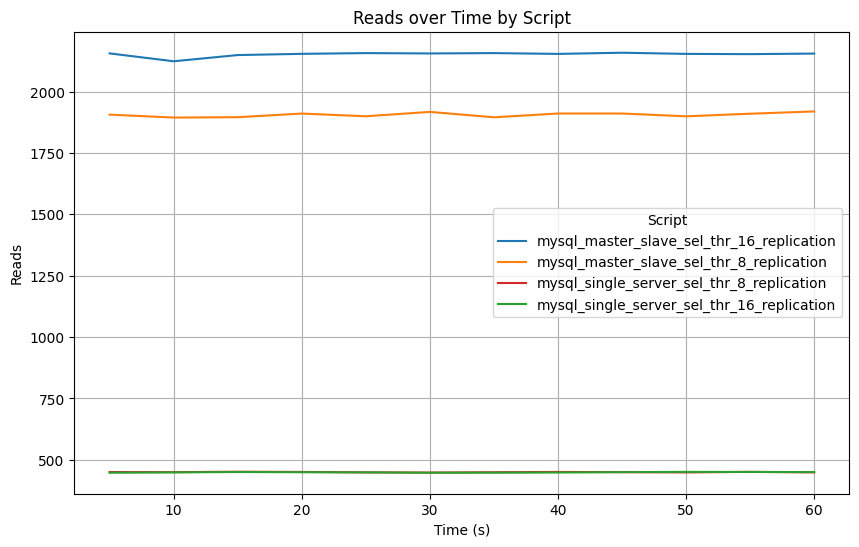
\includegraphics[width=\textwidth]{PNGs/Script/Replication/replication-multiple-select-threads/Reads}
    \caption{Mit Replikation}
    \label{replication-multiple-select-threads-reads}
  \end{subfigure}
  \hfill
  \begin{subfigure}[t]{0.48\textwidth}
    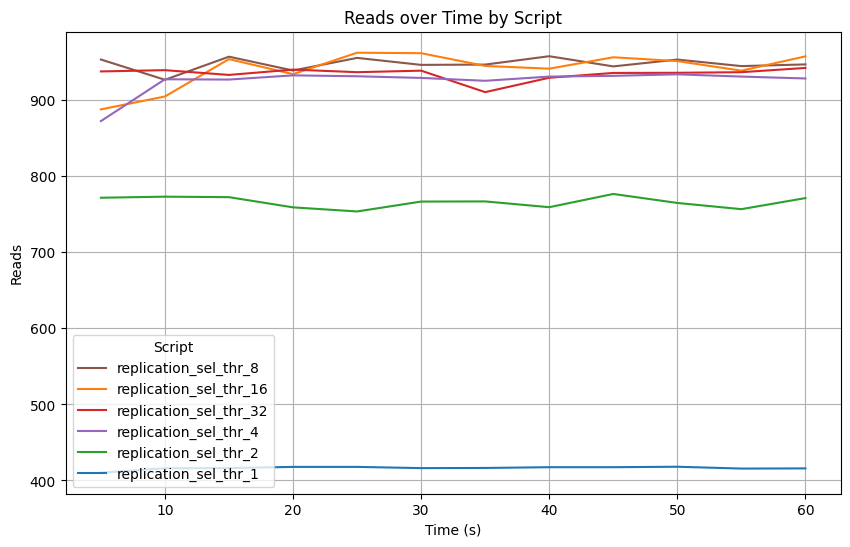
\includegraphics[width=\textwidth]{PNGs/Script/Replication/replication-no-multiple-select-threads/Reads}
    \caption{Ohne Replikation}
    \label{replication-no-multiple-select-threads-reads}
  \end{subfigure}
  \vspace{-5pt}
  \caption[Replikation: Threadanzahl aufgeteilt an Master-Replikate]{Vergleich von 8 Threads an Single-Server und jeweils 2 an die unters. Ports }
  \label{fig:replication-multiple-select-threads}
\end{figure}
\vspace{-20pt}

Zunächst erkennen in der linken Grafik, dass beide Kurven des Single-Server-Ansatzes sehr ähnlich verlaufen.
Auf den ersten Blick könnte das überraschen, da man erwarten würde, dass eine Verdopplung der Threadanzahl auch zu einer Verdopplung der Leseabfragen führt.
Deshalb haben wir noch einen weiteren Vergleich durchgeführt, bei dem wir die Threadanzahlen der 2-er Potenzreihe bis einschließlich $2^5$ nur für den Single-Server-Ansatz getestet haben.
Zusätzlich haben wir bei diesem Vergleich die CPU-Auslastung mit dem folgenden Befehl gemessen:

\vspace{-5pt}
\begin{lstlisting}[language=bash,caption=Messen der CPU-Auslastung,label={lst:replication-cpu-usage},style=custom_daniel,basicstyle=\ttfamily\scriptsize]
top -l 1 | grep 'CPU usage' | awk '{print $3 + $5}' %Für Mac
top -bn1 | grep 'Cpu(s)' | sed 's/.*, *\\([0-9.]*\\)%* id.*/\\1/' | awk '{print 100 - $1}' %Für Linux
\end{lstlisting}
\vspace{-5pt}

Die Ergebnisse der CPU-Auslastung und der Anzahl der Leseabfragen sind in Tabelle~\ref{tab:replication-multiple-select-threads} dargestellt, sortiert nach aufsteigender Threadanzahl.
Die Abbildung~\ref{replication-no-multiple-select-threads-reads} zeigt, dass sich die Leseperformance beim Anstieg von 1 auf 2 Threads nahezu verdoppelt.
Zwischen 2 und 4 Threads fällt der Unterschied schon geringer aus, liegt aber dennoch bei etwa 40\%.
Die restlichen Threadanzahlen weichen nur geringfügig voneinander ab.
Begründen lässt sich das durch die CPU-Auslastung.
Bei geringeren Anzahlen an Threads ist die CPU-Auslastung sehr gering, weshalb wir diese starken Anstiege sehen.
Irgendwann ist die CPU jedoch voll ausgelastet, sodass die Performance nicht mehr weiter steigt.
Dies ist bei 8 Threads der Fall, da dort die CPU-Auslastung bei 89.34\% liegt.

\vspace{-2pt}
\begin{table}[H]
  \centering
  \scriptsize
  \begin{tabular}{|l|l|l|}
    \hline
    \textbf{Anzahl an Threads} & \textbf{Durchschnittliche CPU-Auslastung} & \textbf{Anzahl an Leseabfragen} \\
    \hline
    1 & 1.36\% & 2437 \\
    2 & 26.44\% & 4662 \\
    4 & 67.12\% & 6609 \\
    8 & 89.34\% & 7106 \\
    16 & 85.74\% & 7362 \\
    32 & 99.14\% & 7295 \\
    \hline
  \end{tabular}
  \vspace{3pt}
  \caption{Auslastung mit unterschiedlichen Threadanzahlen}
  \label{tab:replication-multiple-select-threads}
\end{table}
\vspace{-25pt}

Wenn wir jetzt wieder das Ergebnis aus~\ref{fig:replication-multiple-select-threads} betrachten, fallen die Vorteile der Replikation deutlich auf.
In beiden Fällen liegen die Werte mit Replikation stets deutlich über denen des Single-Server-Ansatzes.
Die Performance des Single-Servers bleibt unabhängig von der Threadanzahl nahezu konstant.
Bei der Replikation zeigt sich, dass ein Anstieg an Threads auch zu einer Steigerung der Leseabfragen führt.
So ist die Kombination von 16 Threads, verteilt auf den Master und 3 Replikate, am effizientesten.
Danach folgt mit etwas Abstand die Version mit 8 Prozessen, die etwa 25\% langsamer ist.
Dennoch sind selbst diese deutlich schneller als alle Varianten des Single-Server-Ansatzes, weshalb wir sagen können, dass die Replikation bei höherer Last deutliche Vorteile bringt.

Im letzten Vergleich verwenden wir ausschließlich den Master-Replikat-Ansatz und vergleichen die unterschiedlichen Binlog-Formate, die wir aus~\ref{lst:replication-change-format} kennen.
Um Variationen zu begrenzen, betrachten wir nur ein Replikat pro Master.
Daraus ergeben sich sechs unterschiedliche Leseergebnisse, da für jedes der drei Formate sowohl der Master- als auch der Replikat-Port abgefragt wird.
In der Grafik~\ref{fig:replication-format-change} können wir sehen, dass es bei den verschiedenen Binlog-Formaten und Ports kaum Unterschiede zu erkennen gibt.
Und auch die Schreibgeschwindigkeiten verhalten sich bei beiden Varianten sehr ähnlich.
Das können wir auch mit dem Hexagon-Chart bestätigen, da dort alle Werte sehr nah beieinander liegen.

\begin{figure}[H]
  \centering
  \begin{subfigure}[t]{0.48\textwidth}
    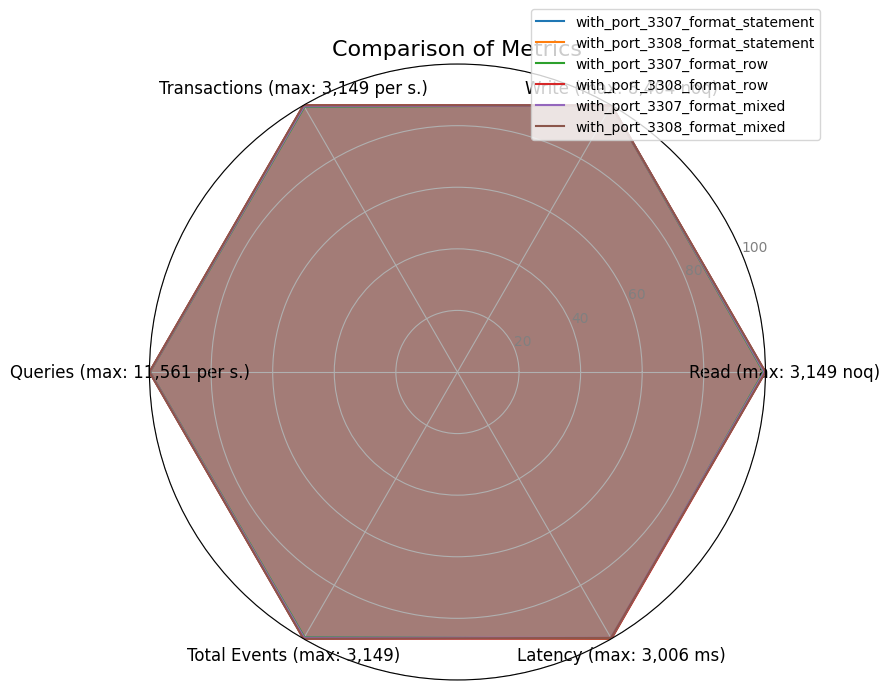
\includegraphics[width=\textwidth]{PNGs/Script/Replication/replication-format-change/statistics}
  \end{subfigure}
  \hfill
  \begin{subfigure}[t]{0.48\textwidth}
    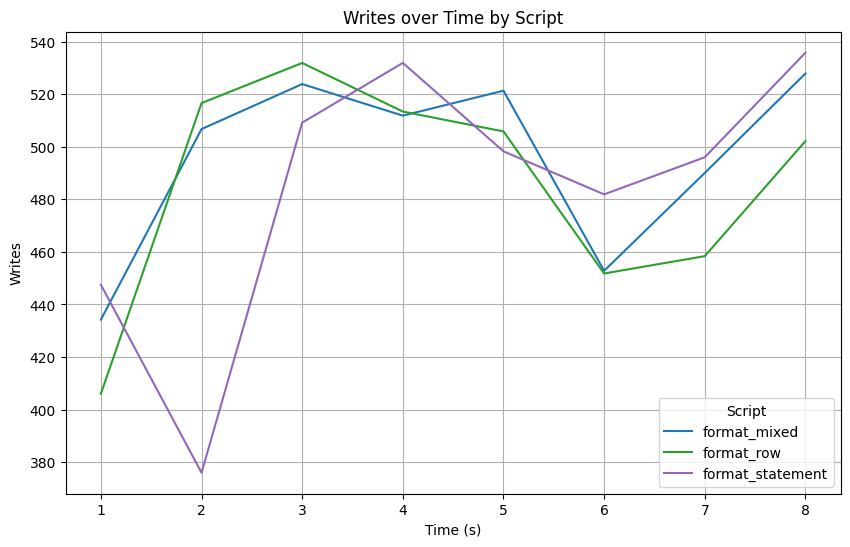
\includegraphics[width=\textwidth]{PNGs/Script/Replication/replication-format-change/Writes}
  \end{subfigure}
  \vspace{-8pt}
  \caption[Replikation: Unterschiedliche Binlog-Typen]{Vergleich zwischen den unterschiedlichen Binlog-Typen }
  \label{fig:replication-format-change}
\end{figure}
\vspace{-20pt}

Die Schlussfolgerungen, die wir aus den Messungen gewinnen können, sehen dabei wie folgt aus.
Wir sehen, dass durch Replikation, anders als beispielsweise mit Indexen oder Partitionen, bei einem einzelnen Thread keine deutlichen Performancevorteile gewonnen werden können.
Wenn aber mehrere Nutzer auf der Datenbank interagieren und ausschließlich Lesezugriffe benötigen, dann können die Abfragen auf die unterschiedlichen Ports aufgeteilt werden.
In diesen Szenarien mit höherer Parallelität und intensiveren Leseoperationen kann Replikation daher signifikante Vorteile bieten.
Die Auswahl des Binlog-Formats hat bei unserem Benchmark zu keinen Performanzgewinnen geführt.
Möglicherweise könnte sich jedoch ein anderer Einfluss zeigen, wenn Schreiboperationen ins Spiel kommen oder die Konsistenzanforderungen geändert werden.
